\section{Experimental Evaluation}\label{sec:experiments}

In this section we quantify some aspects of our implementation.
Looking at Figure~\ref{fig:adapters}, it is clear that data crosses
many layers.  In this section we strictly evaluate the performance of
the central block, the \dbsp query engine.  However, in most real-life
application performance will be limited by the adapters and network
communication.

\subsection{Latency, throughput, and input change size}

Latency is the time between submitting a change and obtaining a
result.  Observed latency is a function of both query complexity and
the size of the internal state, so latency will change as a system
state grows.

For relatively simple queries, as described in
Section~\refsec{sec:macrobenchmarks}, while running in steady state,
the latency of a transaction changing a single input row is on the
order of tens to hundreds of microseconds, proving that our engine can
be used for very low latency applications.

Throughput is the number of records that can be processed in a time
unit.  \dbsp is synchronous and blocking model: for every input
change, the pipeline does not accept any other inputs until it has
produced the output for all views.  This suggests that latency is the
inverse of throughput.

There is an additional degree of freedom: the size of an input
transaction.  In several scenarios there is a choice: (1) when a
pipeline is started and is ingesting the initial state of a large
database (\emph{backfilling}), or (2) when processing data from
streaming sources, without clear transaction boundaries.

As Nikolic has observed before~\cite{nikolic-sigmod16}, there is a
relatively tight relationship between the latency of updating a view,
the throughput, and the size of the input changes.  Nikolic finds that
in DBToaster the optimal value is somewhere between 1K and 10K tuples.
Our experiments confirm this.  The exact optimum value depends on the
query and data distribution.  Figure~\ref{fig:batchsize} shows some
typical measurements for Nexmark query Q5.  Latency grows
monotonically with input batch size, but the optimum throughput is
obtained for batches of 2K-20K records.

\begin{figure}[h]
  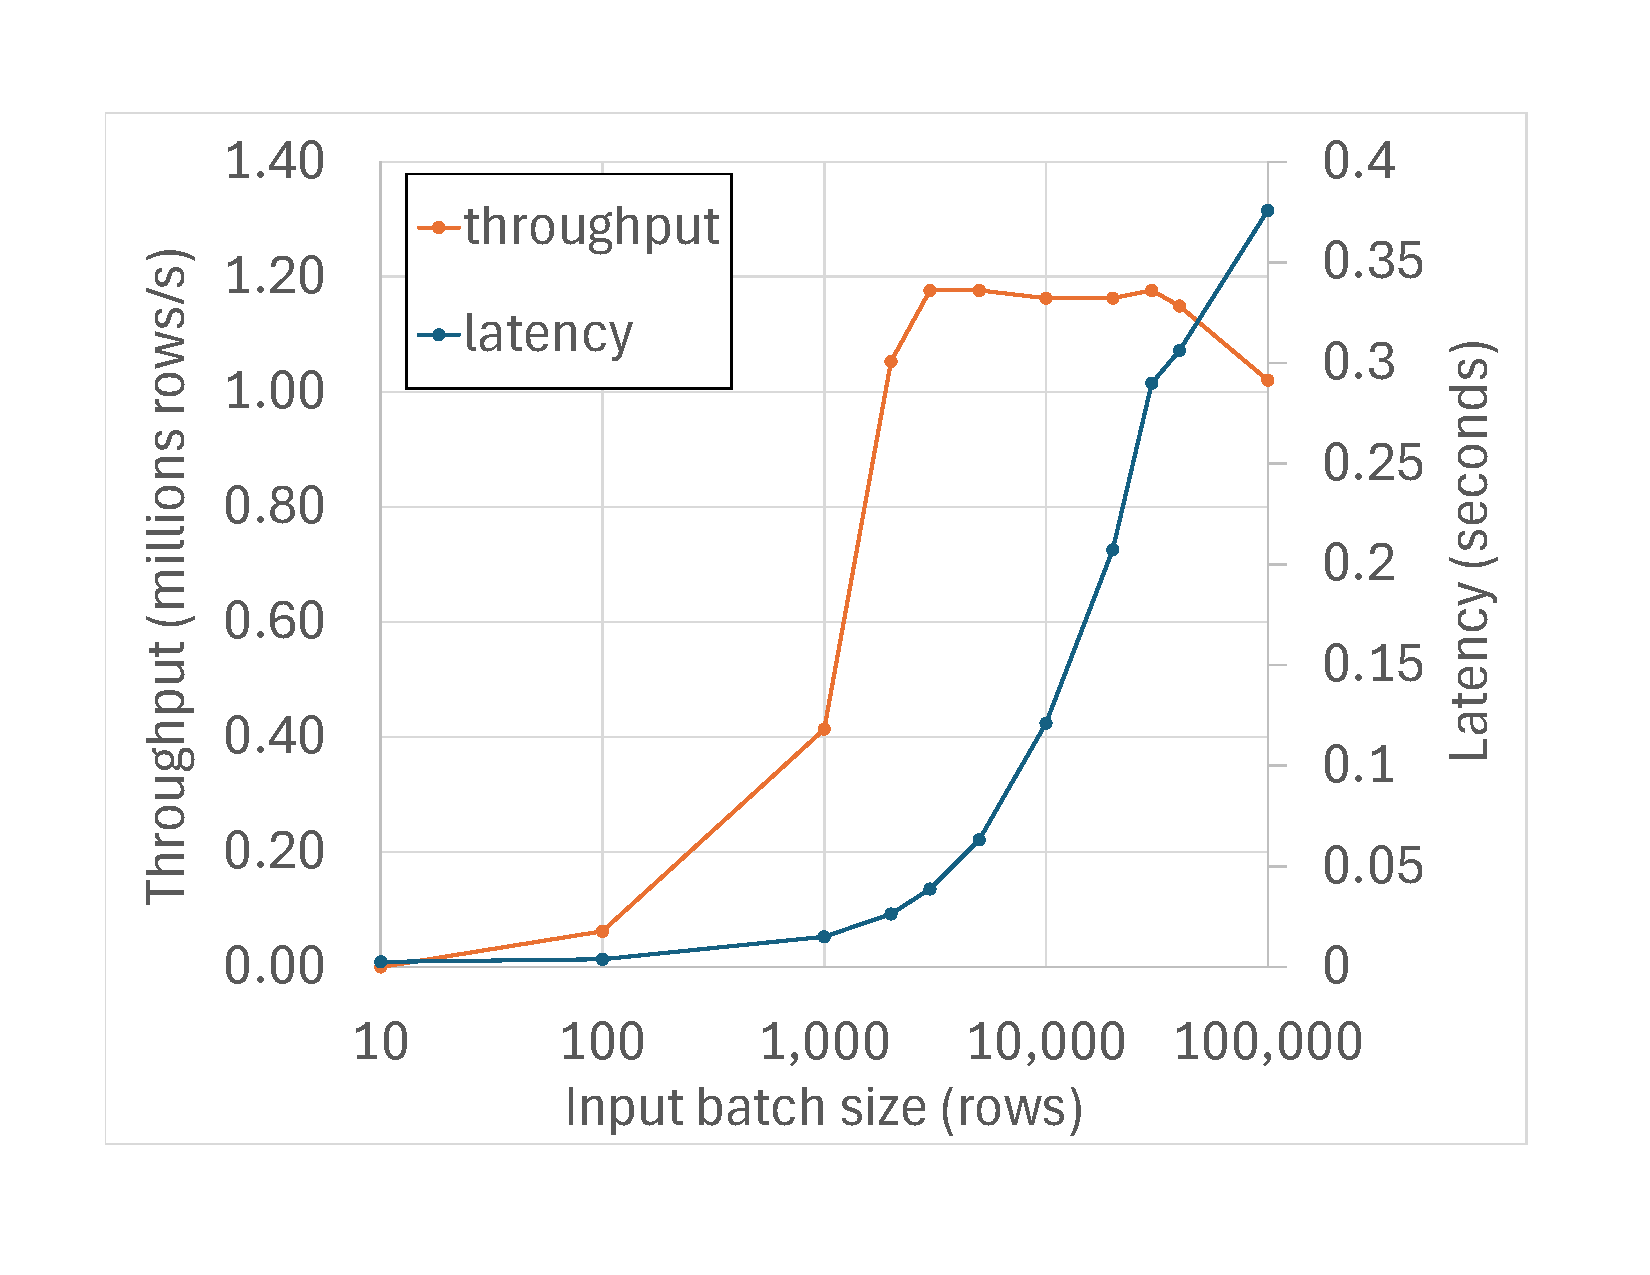
\includegraphics[width=.90\columnwidth]{graph/batchsize}
  \caption{Latency and throughput as a function of the input batch
    size.  Notice the logarithmic X axis.\label{fig:batchsize}}
\end{figure}

Increasing the batch size further beyond 100K records causes the
system to enter an unstable state (the crossover point depends on the
available memory size), in which throughput oscillates, as shown in
Figure~\ref{fig:oscillation}.  One reason this happens is that some
activities, such as merging batches, and garbage-collection of useless
records, only happen between circuit steps.  The right solution to
smooth these oscillations is probably a dynamic controller for input
sizes, but also for partitioning resources like memory between \dbsp
operators and their shards.

\begin{figure}[h]
  \begin{center}
  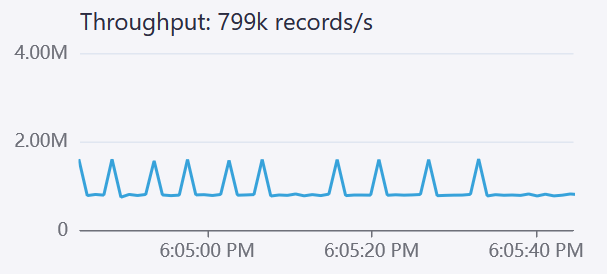
\includegraphics[scale=.5]{graph/oscillation}
  \caption{Unstable throughput for very large input batch
    sizes\label{fig:oscillation}.}
  \end{center}
\end{figure}

\subsection{Macrobenchmarks}\label{sec:macrobenchmarks}

\begin{figure*}
  (a) 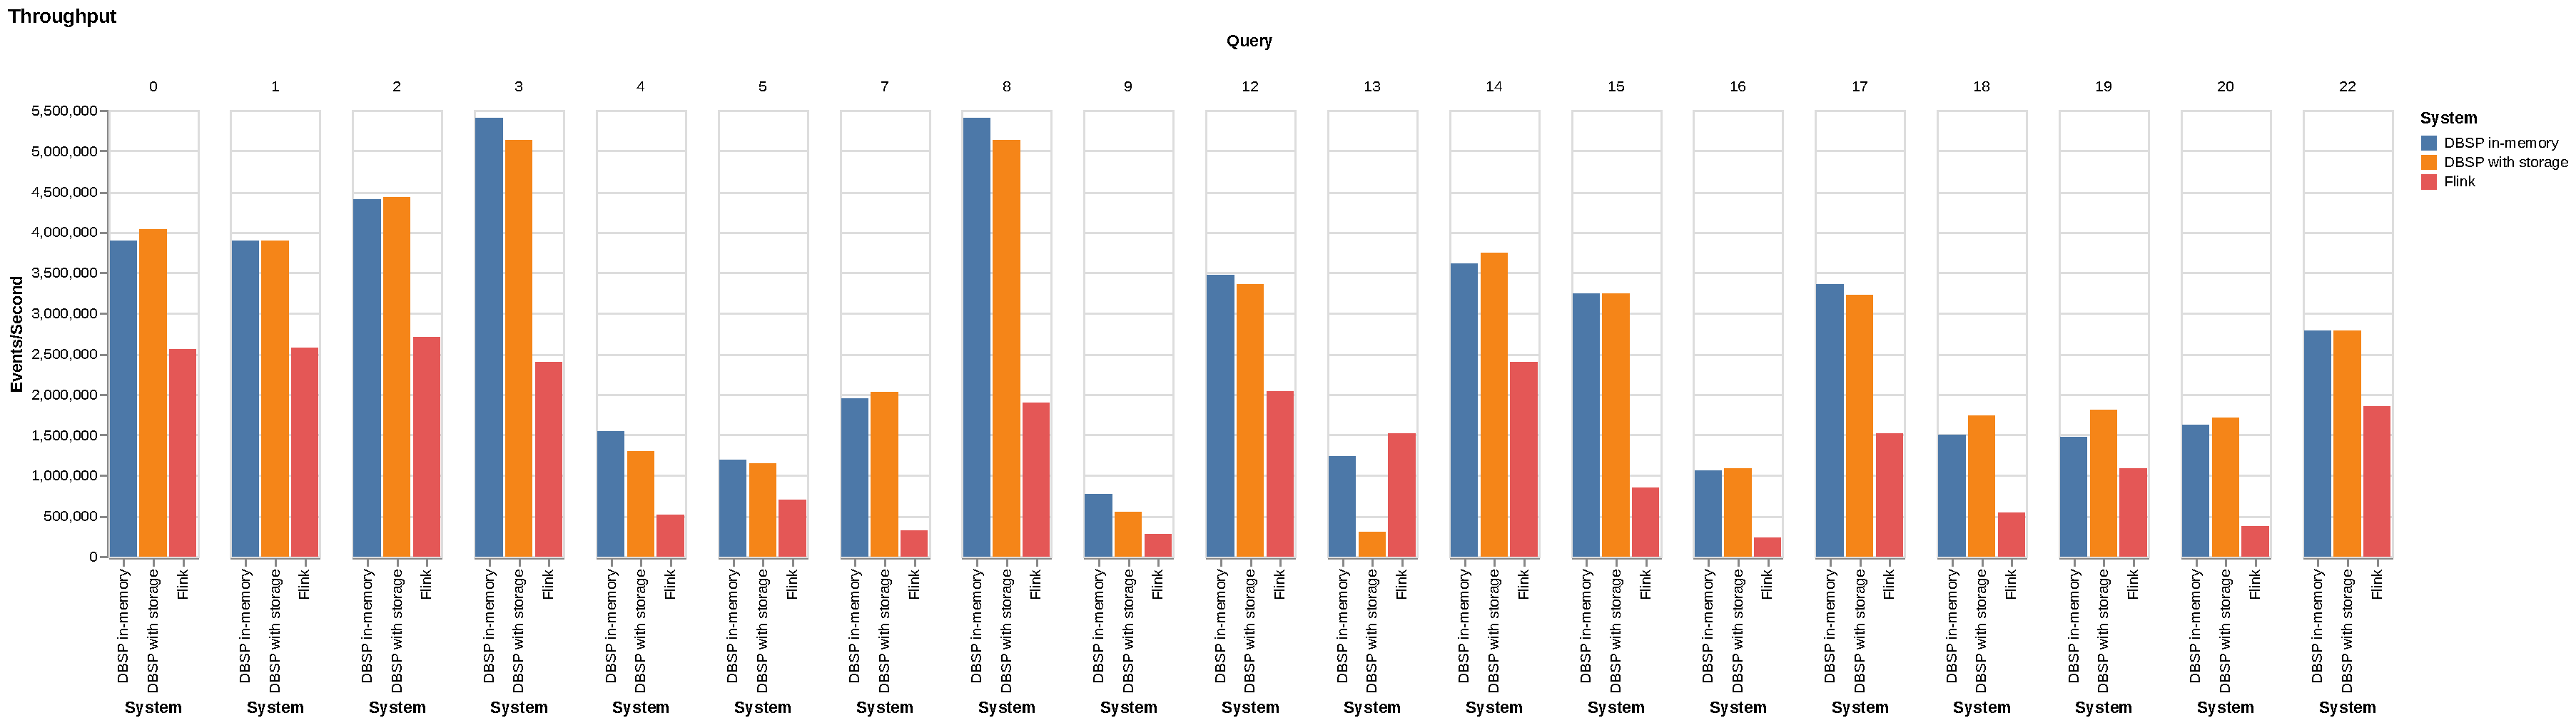
\includegraphics[width=.95\textwidth]{graph/throughput} \\
  (b) 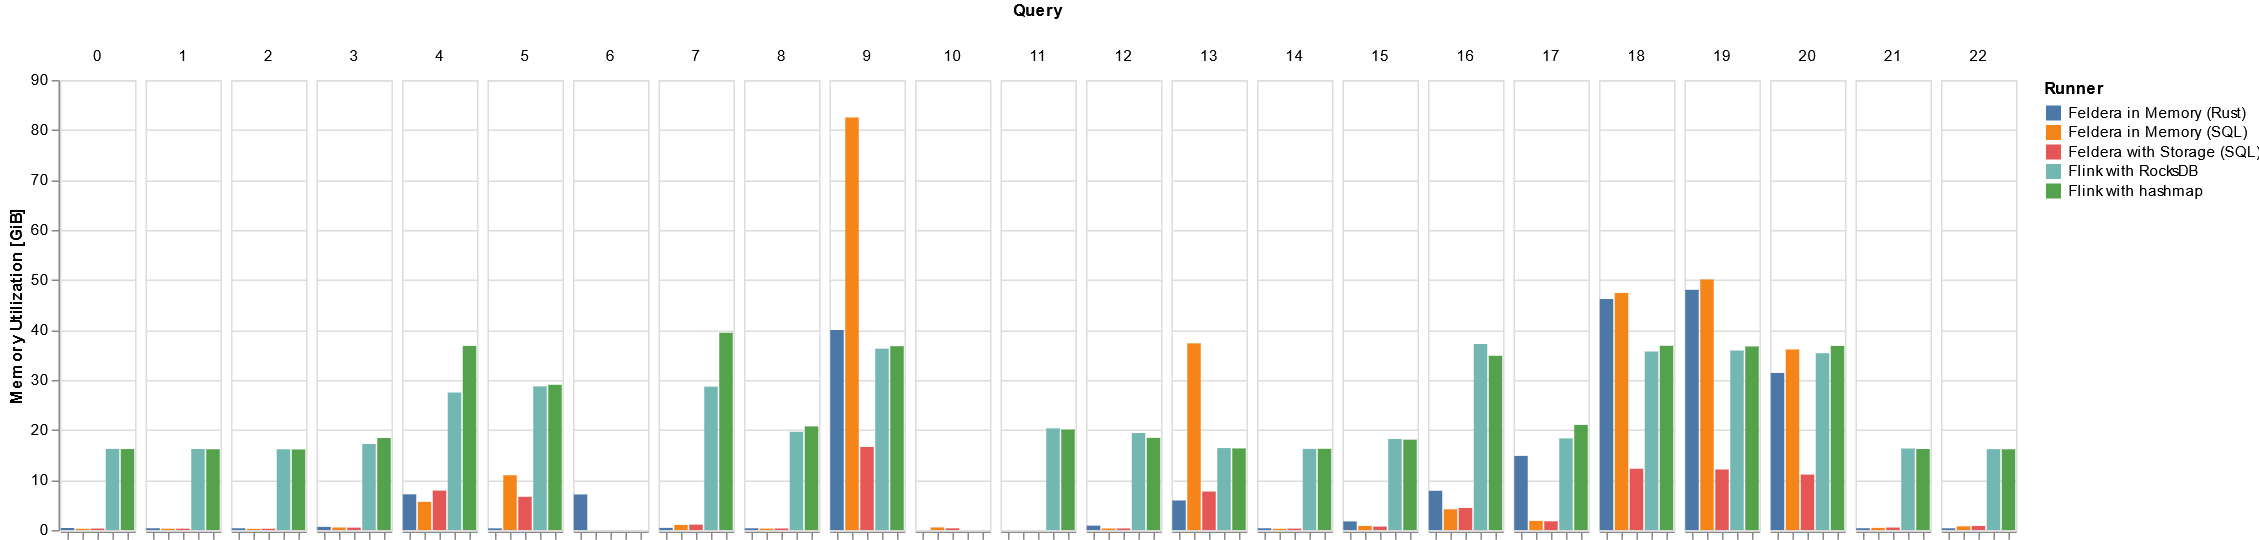
\includegraphics[width=.95\textwidth]{graph/memory} \\
  \caption{(a) Average throughput, in events processed per second
    (higher is better), and (b) peak memory consumption (lower is
    better), in GiB (\(2^{30}\) bytes).  The workload comprises the
    Nexmark queries that DBSP and Flink support in common, over
    100,000,000 events.\label{fig:macrobenchmark}}
\end{figure*}

\newcommand{\query}[1]{\textsf{#1}}

There are no standard benchmark suites for IVM.  In this section we
use an atypical benchmark suite, Nexmark~\cite{tucker2008nexmark},
which was designed for benchmarking streaming systems.  The benchmark
is driven by a synthetic data generator, modeling for an online
auction site along with a suite of queries against the streams.
Nexmark is already implemented for other streaming database systems,
notably for Flink~\cite{carbone-ieee15,nexmark-flink}, a widely used
stream processing system.

We compare \dbsp against Flink on the Nexmark benchmark, which
consists of 23 queries.  We use the queries that the Flink and \dbsp
implementations have in common.  We omitted \query{q6} because there
was no Flink implementation, and \query{q10} because we could not make
Flink's implementation for it work.  We omitted \query{q11} and
\query{q21} because DBSP does not yet support session windows and
user-defined functions\footnote{The latter feature is expected to be
ready soon.}.

We ran both the Flink and \dbsp implementations on the same machine,
which has a 64-core, 128-thread Threadripper~3990X CPU and 256~GB RAM,
with Fedora Core~40 as the operating system. We present results for
100~million Nexmark events (input records), which is a moderate
number.

\dbsp runs as a single process with 16~worker threads, and otherwise
with default settings.  We ran \dbsp both with storage disabled, where
\dbsp keeps all state in RAM, and with storage enabled, where \dbsp
flushes state to secondary storage as it gets large
(see~\ref{sec:state-management}).  Enabling storage allows \dbsp to
work with more state with less memory use, at some cost in throughput.

We configured the Flink implementation of Nexmark with the settings
recommended by the upstream project, running 8~Flink task manager
containers, each allocated 2~cores, and one Flink job manager
container.  We tried adjusting Flink and Nexmark settings, but none of
these changes improved Flink performance in a significant and
reproducible way.

\dbsp and Flink support reading input from multiple kinds of data
sources.  For these measurements, we configured both of them to use
their own integrated Nexmark event generators, rather than pulling
them from Kafka or HTTP or another source.  This eliminated network
service performance and configuration as a possible source of
variability.

Figure~\ref{fig:macrobenchmark} reports our measurements.  The two
bars for \dbsp in each case report results with and without enabling
secondary storage.

\paragraph{Throughput.}

\newcommand{\x}{\(\times\)}

Figure~\ref{fig:macrobenchmark}(a) shows throughput of \dbsp versus
Flink.  In-memory we are up to 6.2\x{} faster than Flink, with a
geometric mean of 2.2\x{} faster on average.  As queries get more
complicated, \dbsp's advantage over Flink grows by a much larger
factor.  For example, \query{q7} is 6.2\x{} faster in \dbsp vs. Flink,
and q16 and q20 are about 4.5\x{} faster.

\query{q13} is an outlier that performs slightly slower in out system
than Flink; with storage enabled, it is slower than Flink.  With
\query{q13} excluded, every remaining query runs at least 1.4\x{}
faster in Feldera (with or without storage).  We are investigating
this behavior.

Storage generally has a small impact on our throughput, except for
\query{q13}, where it has about a 4\x{} penalty.  \query{q0} and other
very simple queries are about 1.5\x{} faster.

\paragraph{Peak memory.}

Figure~\ref{fig:macrobenchmark}(b) shows peak memory consumption, as
reported as the operating system RSS (resident set size), for the
Flink or Feldera processes.  In our case this is a single process; for
Flink, it is the sum of the RSS in the 8 task manager containers.  We
did not include the control plane in either case (in Feldera's system,
the pipeline manager; in Flink, the job manager).

We use between 0.03\x{} and 2.6\x{} as much memory of Flink, with a
geometric mean of 0.24\x{}.

\query{q0} and several other queries use 2~GiB or less memory with our
implementation, but over 17~GiB with Flink.  These queries are linear,
and do not require any state, or only minimal state, so it does not
allocate much memory.  Flink runs under the Java Virtual Machine,
which might cause it to allocate a high minimum amount of memory.

Most queries use less memory in our system than in Flink.  \query{q9}
and \query{q13} use substantially more, and \query{q18} and
\query{q19} use somewhat more, and storage reduces the storage
significantly.
